\part{DC machines}
\title{DC machines}  
\date{}  
\frame{\titlepage} 

%%%%%%%%%%%%%%%%%%%%%%%%%%%%%%%%%%%%%%%%%%%%%%%%%%%%%%%%%%%%%
%% Homopolar / unipolar machines %%
%%%%%%%%%%%%%%%%%%%%%%%%%%%%%%%%%%%%%%%%%%%%%%%%%%%%%%%%%%%%%
\begin{frame}
	\frametitle{Homopolar / unipolar machines}
    \vspace{-0.3cm}
	\begin{figure}
		\centering
		\begin{subfigure}[b]{0.49\textwidth}
			\centering
			\movie{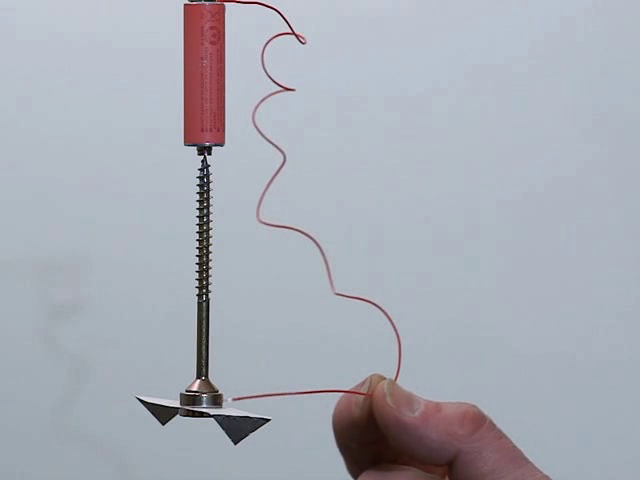
\includegraphics[height=0.4\textheight]{fig/lec03/homopolar_machine_video.png}}{fig/lec03/homopolar_machine_video.mp4}
            \vspace{0.75cm}
			\caption{Video of an operating homopolar machine (source: \href{https://de.wikipedia.org/wiki/Datei:Homopolarmotor_MAQ03891_smial_wp.ogv}{Wikimedia Commons}, Smial, \href{https://artlibre.org/licence/lal/en/}{Free Art License})}
		\end{subfigure}
		\hfill
		\begin{subfigure}[b]{0.49\textwidth}
			\centering
			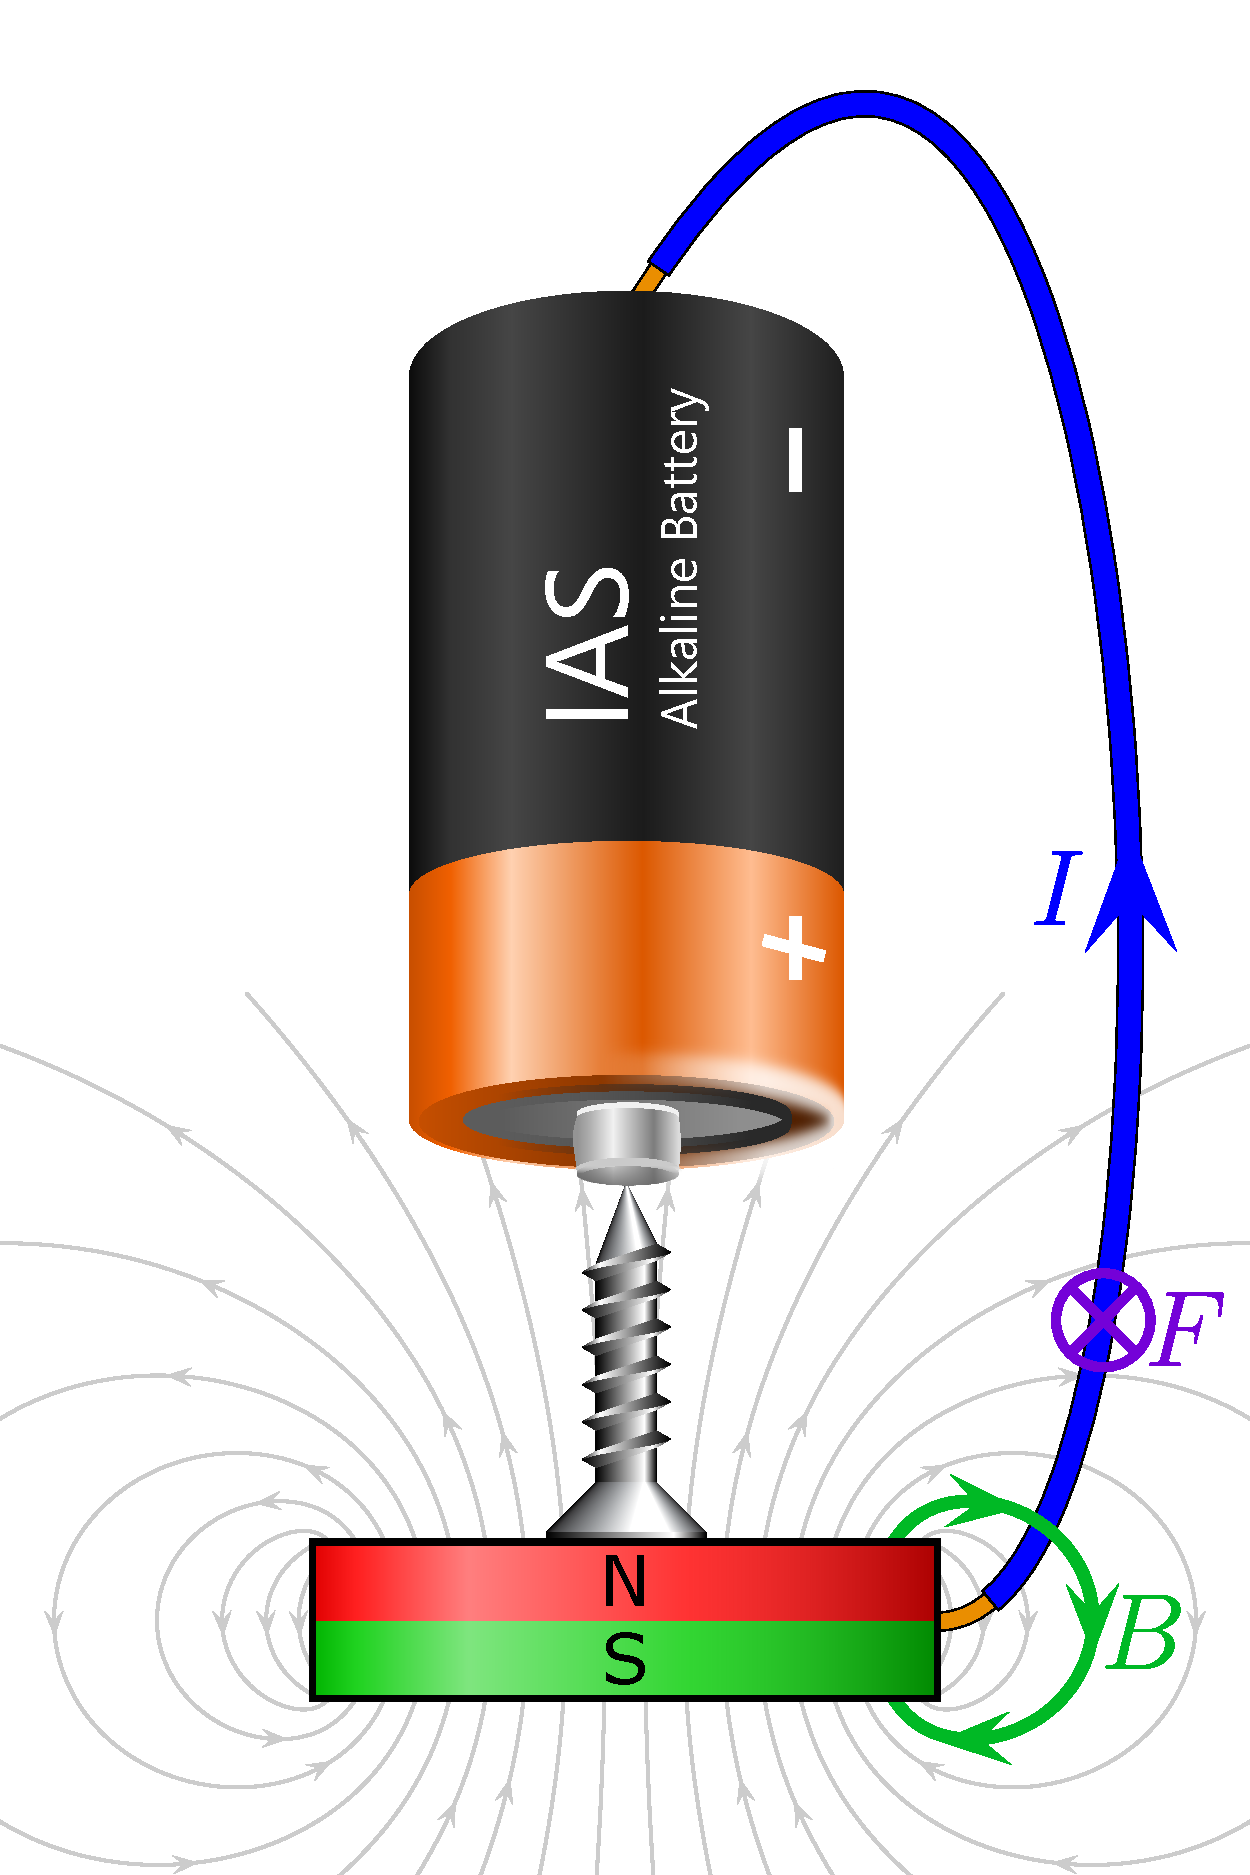
\includegraphics[width=0.47\textwidth]{fig/lec03/Homopolar_machine.pdf}
			\caption{Electric current, magnetic field and Lorentz force (adapted: \href{https://commons.wikimedia.org/wiki/File:Homopolar-motor.svg}{Wikimedia Commons}, M. Run, \href{https://creativecommons.org/licenses/by-sa/4.0/deed.en}{CC BY-SA})}
		\end{subfigure}
		\caption{Working principle of homopolar machines demonstrated with a simple permanent magnet, battery and screw design} 
        \label{fig:Homopolar_machine}
	\end{figure}
\end{frame}


%%%%%%%%%%%%%%%%%%%%%%%%%%%%%%%%%%%%%%%%%%%%%%%%%%%%%%%%%%%%%
%% Homopolar / unipolar machines (cont.) %%
%%%%%%%%%%%%%%%%%%%%%%%%%%%%%%%%%%%%%%%%%%%%%%%%%%%%%%%%%%%%%
\begin{frame}
	\frametitle{Homopolar / unipolar machines (cont.)}
    \begin{columns}
		\begin{column}{0.5\textwidth}
            \begin{itemize}
                \item  Homopolar machines are the simplest form of electric machines.
                \item They are also true DC machines, as the current and flux paths are unidirectional.
                \item The general design prevents connecting multiple rotor turns in series to increase the voltage, that is, only a relatively low voltage is induced.
                \item Consequently, homolpolar machines require high currents (in the order of  \si{\kilo\ampere} or even \si{\mega\ampere}) to reach a useful power range which limited their application.
            \end{itemize}
		\end{column}
        \hfill
		\begin{column}{0.49\textwidth}
			\begin{figure}
				\centering
				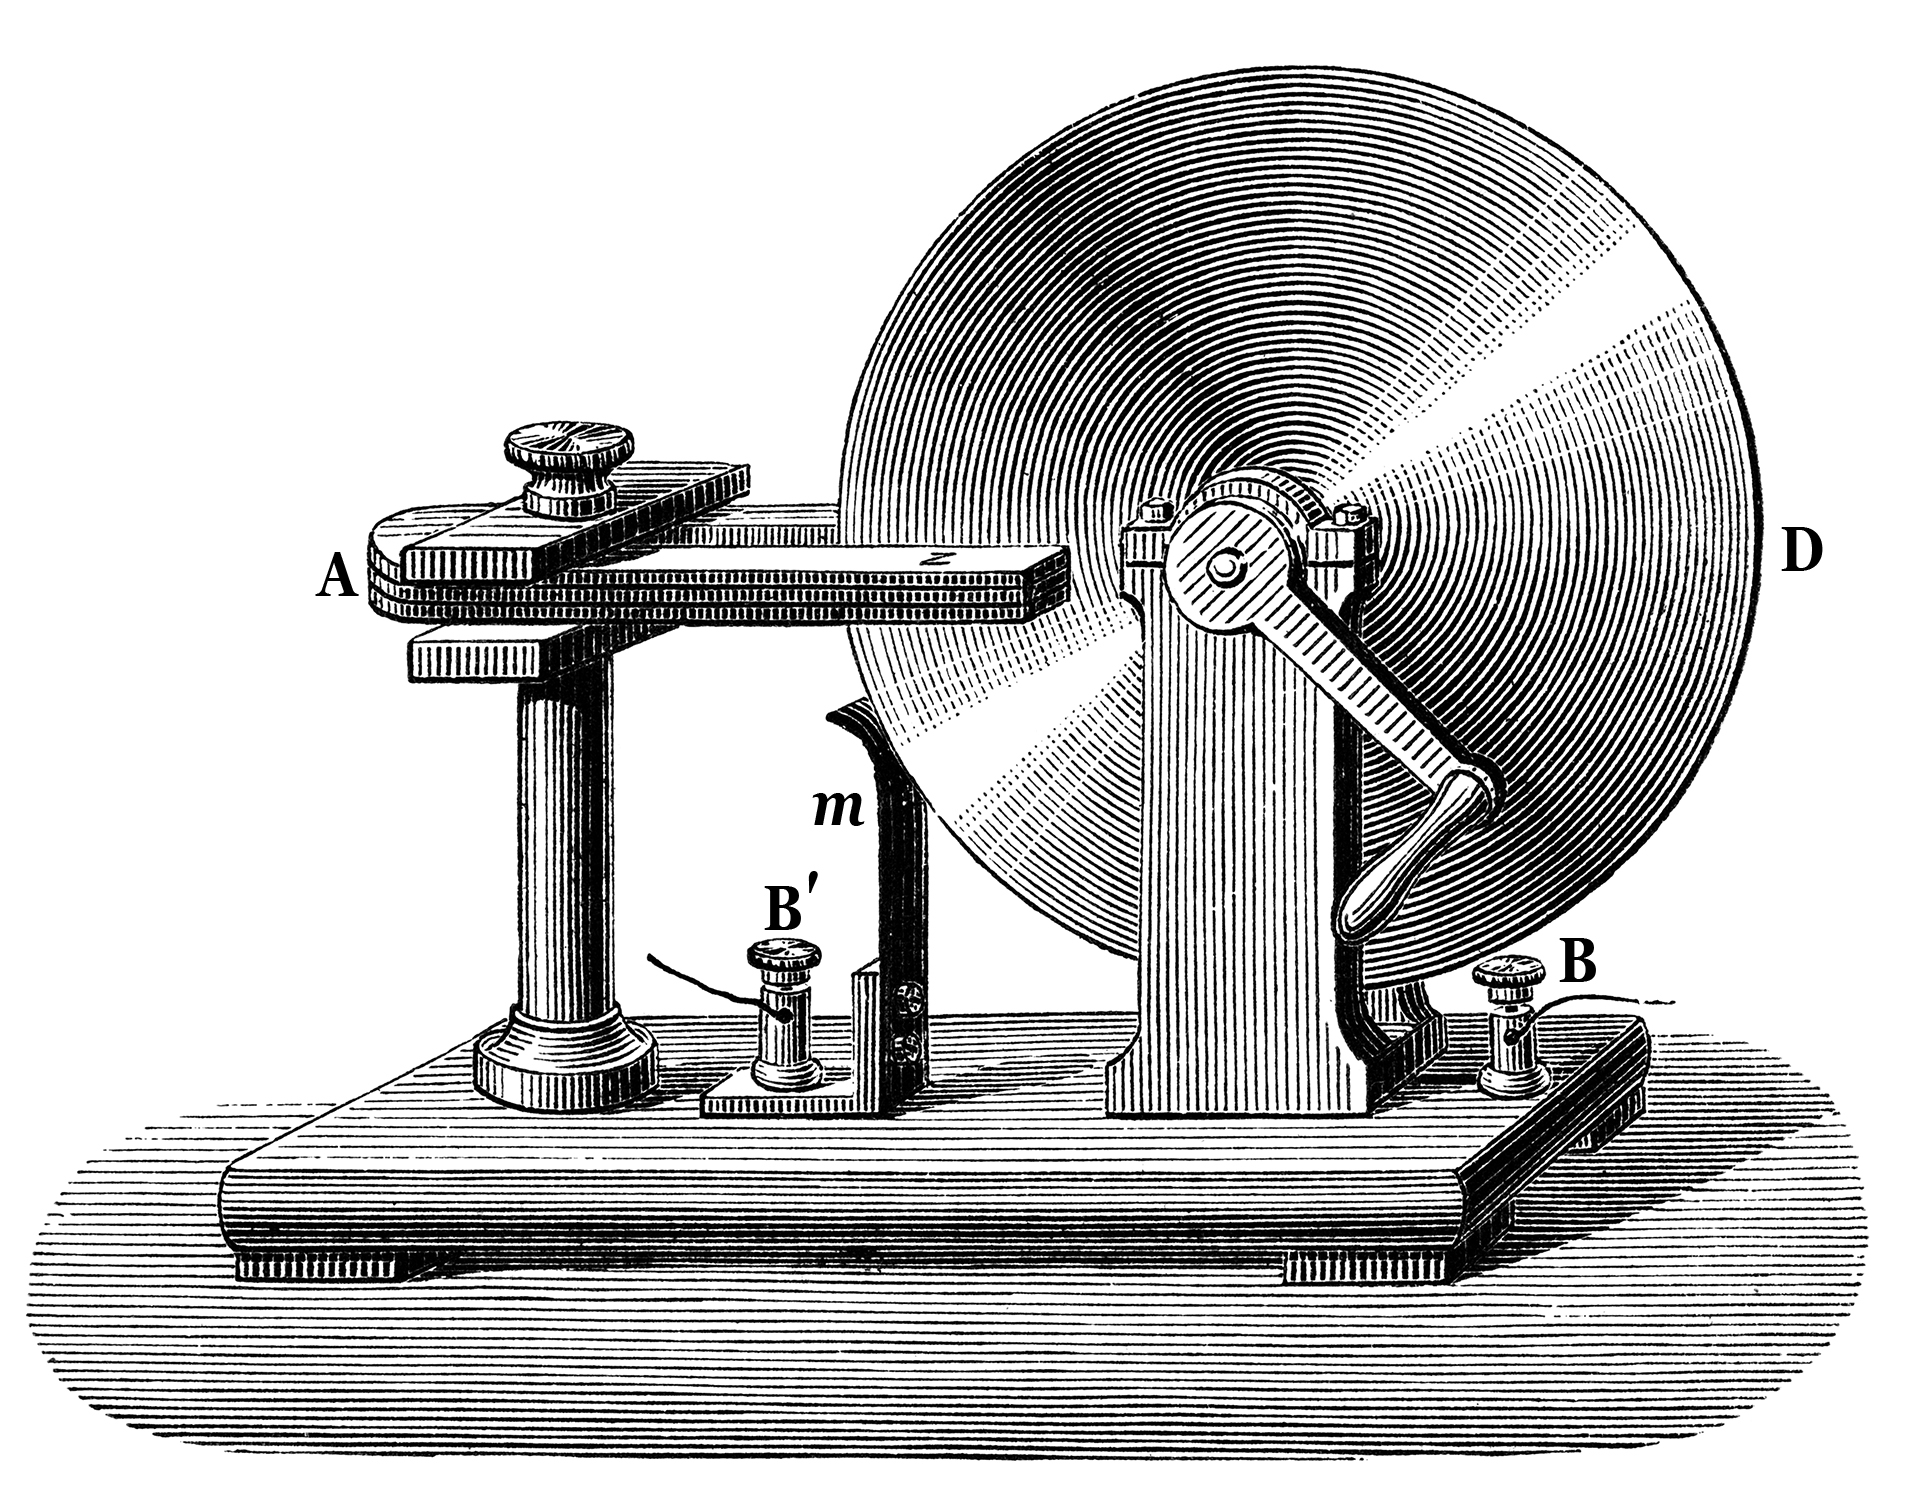
\includegraphics[width=0.8\textwidth]{fig/lec03/Faraday_disk_generator.jpg}
				\caption{The Faraday disk: another homopolar machine (source: \href{https://commons.wikimedia.org/wiki/File:Faraday_disk_generator.jpg}{Wikimedia Commons}, Public domain)}
			\end{figure}
		\end{column}
		\end{columns}
\end{frame}

%%%%%%%%%%%%%%%%%%%%%%%%%%%%%%%%%%%%%%%%%%%%%%%%%%%%%%%%%%%%%
%% Working principle of usual DC machines %%
%%%%%%%%%%%%%%%%%%%%%%%%%%%%%%%%%%%%%%%%%%%%%%%%%%%%%%%%%%%%%
\begin{frame}
	\frametitle{Working principle of usual DC machines}
    \begin{columns}
		\begin{column}{0.5\textwidth}
            Let's consider \figref{fig:Simple_yoke_coil} and assume that the flux density $B$ is constant in the air gap and that the conductor loop has a length $l$. According to the Lorentz force we have
			\begin{equation}
				F = i_\mathrm{A} B l .
			\end{equation}  
			The torque $T$ on the conductor loop is given by
			\begin{equation}
				T = 2 F \frac{d}{2} \cos\alpha r = i_\mathrm{A} B l d \cos\left(\alpha\right).
			\end{equation}
			If the coils spins with an angular velocity $\omega$, mechanical power $P_\mathrm{me} = T\omega$ is produced. 
			\\[1em]
			\textbf{Question:} What is happening if the coil is outside the magnetic field?
		\end{column}
        \hfill
		\begin{column}{0.49\textwidth}
			\begin{figure}
				\centering
				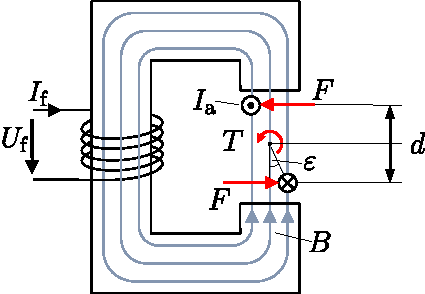
\includegraphics[width=0.9\textwidth]{fig/lec03/Simple_yoke_coil.pdf}
				\caption{Torque on a conductor loop (adapted from J.~B\"ocker, \textit{Elektrische Antriebstechnik}, Paderborn University, 2020)}
				\label{fig:Simple_yoke_coil}
			\end{figure}
		\end{column}
		\end{columns}
\end{frame}